\chapter{DESIGN ANALYSIS}\label{design analysis}
\thispagestyle{empty}

As mentioned in the Section \ref{chap2}, the proposed vending machine accepts used plastic pens instead of coins. The used pen will be deposited through the top portion of PPVM. A rubber flap will be provided which will automatically open and close when the pen is inserted. A barrier will be provided below the flap which can be used to block the entry of the pen when the machine is off. Once the pen is dropped, it falls into a transparent box. This box is attached to a base that can tilt in two directions. The object is accepted or rejected after the image processing.

\section{Image capture}
A camera attached inside the machine scans the transparent box. It takes an image and sends it to the processor of the machine. For the prototype, a Raspberry Pi 3b was used. The processor uses pattern recognition and image classification to determine whether the object inserted is a pen or not. If it is a pen, the processor sends a signal to the tiltable base and the pen is redirected to the storage bin inside the machine. If it is not a pen, then the base ejects the object out of the machine. After insertion of three pens into the machine, a signal is sent to the rotating delivery system that will roll out one pen and deliver it to the user.

\section{Image recognition and classification}
The image capture and manipulation was done with the help of a python library called Open-source Computer Vision or OpenCV \cite{opencv}. For the recognition process, ``TensorFlow" was used, as mentioned in Section \ref{tf_sec}. Using a training dataset consisting of images of pens, a model pattern of a pen was created. This model is then compared with a trial dataset to determine the accuracy of the model. If the accuracy is low, the model is re-trained. The camera takes a picture of the waste pen and adds it to the test dataset. Once recognized, the image is properly labeled, either ``pen" or ``not pen", and then adds this to the training dataset. Then the model is retrained. Thus, by implementing machine learning, PPVM will become more and more accurate with each use. See Appendix \ref{code} for the detailed code. An example of the image classification during the testing stage is shown in Fig \ref{clf1}. This algorithm optimized and implemented in the prototype, gave the results as shown in Fig \ref{clf2}. A flowchart showing this algorithm is shown in Fig \ref{flow}.

\begin{figure}[H]
\centering

	\begin{subfigure}[Image classification during tests] 
		{\label{clf1}
			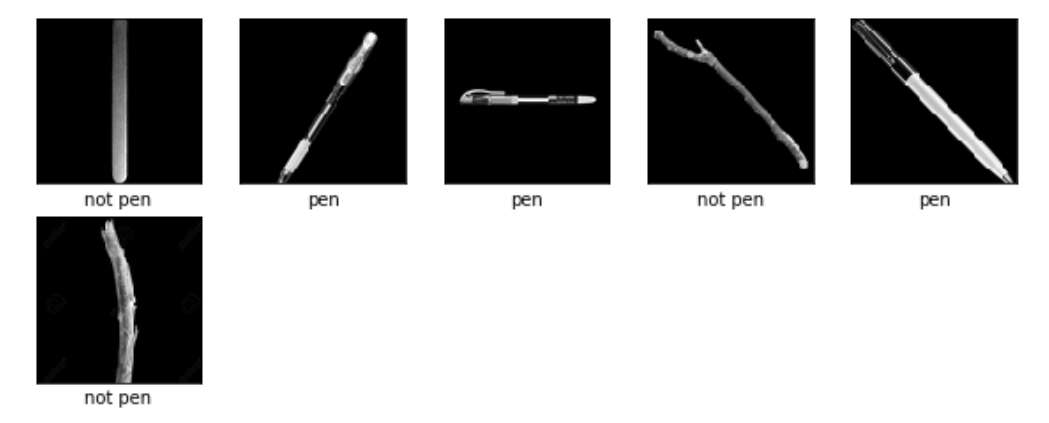
\includegraphics[width=1\textwidth]{./picture-files/imgclf.png}}
	\end{subfigure}\hfill 
	\begin{subfigure}[Image classification implemented in prototype]
		{\label{clf2}
		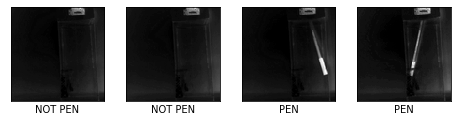
\includegraphics[width=1\textwidth]{./picture-files/imgclf2.png}}
	\end{subfigure}
	\caption{Image recognition and classification algorithm}
\end{figure}

\section{Model Design}

Careful calculations were done for making the prototype. The PPVM needed to be as small as possible and the space needed to be utilised as much as possible. The model drawing of the PPVM is shown in Fig \ref{Model} with all dimensions in inches. The prototype made is shown in Fig \ref{proto}.

\begin{figure}[H]
\centering

\begin{tikzpicture}[node distance=2cm]
\tikzset{minimum size= 1cm}
\node (start) [startstop] {Start};
\node (in1) [io, below of=start, minimum height=0.5cm] {Pen Input to PPVM};
\node (pro1) [process, below of=in1,minimum height=0.5cm] {Image processing};
\node (dec1) [decision, below of=pro1,minimum height=0.5cm, yshift=-0.5cm] {Pen or not};
\node (count) [process, below of=dec1,minimum height=0.5cm, yshift=-0.5cm] {Pen count ++};
\node (dec2) [decision, below of=count,minimum height=0.5cm, yshift=-1.5cm] {No. of pens = 3 or not};
\node (img_yes) [io, left of= dec1, minimum height=0.5cm, xshift=-2.9cm] {Image Input to database};
\node (img_yes2) [io, below of= dec2, minimum height=0.5cm, yshift=-2cm] {Image Input to database};
\node (out1) [io, below of=img_yes2, minimum height = 1cm] {Roll-out Paper Pen};
\node (pro2b) [process, right of=dec1, xshift=3cm] {Reject};
\node (img_no) [io, right of= pro1, minimum height=0.5cm, xshift=3cm] {Image Input to database};

\node (stop) [startstop, below of=out1] {Stop};
\draw [arrow] (start)-- (in1);
\draw [arrow] (in1)  -- (pro1);
\draw [arrow] (pro1) -- (dec1);
\draw [arrow] (count) -- (dec2);
\draw [arrow] (dec2) -- node[anchor=east] {yes} (img_yes2);
\draw [arrow] (dec1) -- (pro2b);

\draw [arrow] (dec1) -- node[anchor=east] {yes} (count);
\draw [arrow] (dec1) -- node[anchor=south] {no} (pro2b);
\draw [arrow] (dec2) -- +(-4,0) -| (img_yes) node[near start,sloped,above] {no};
\draw [arrow] (img_yes) |- (in1);
\draw [arrow] (img_no) |- (in1);
\draw [arrow] (pro2b) -- (img_no);
\draw [arrow] (img_yes2) -- (out1);
\draw [arrow] (out1) -- (stop);
\end{tikzpicture}

\caption{Flowchart showing the algorithm of the PPVM}
\label{flow}
\end{figure}


\begin{figure}[H]
	\centering
	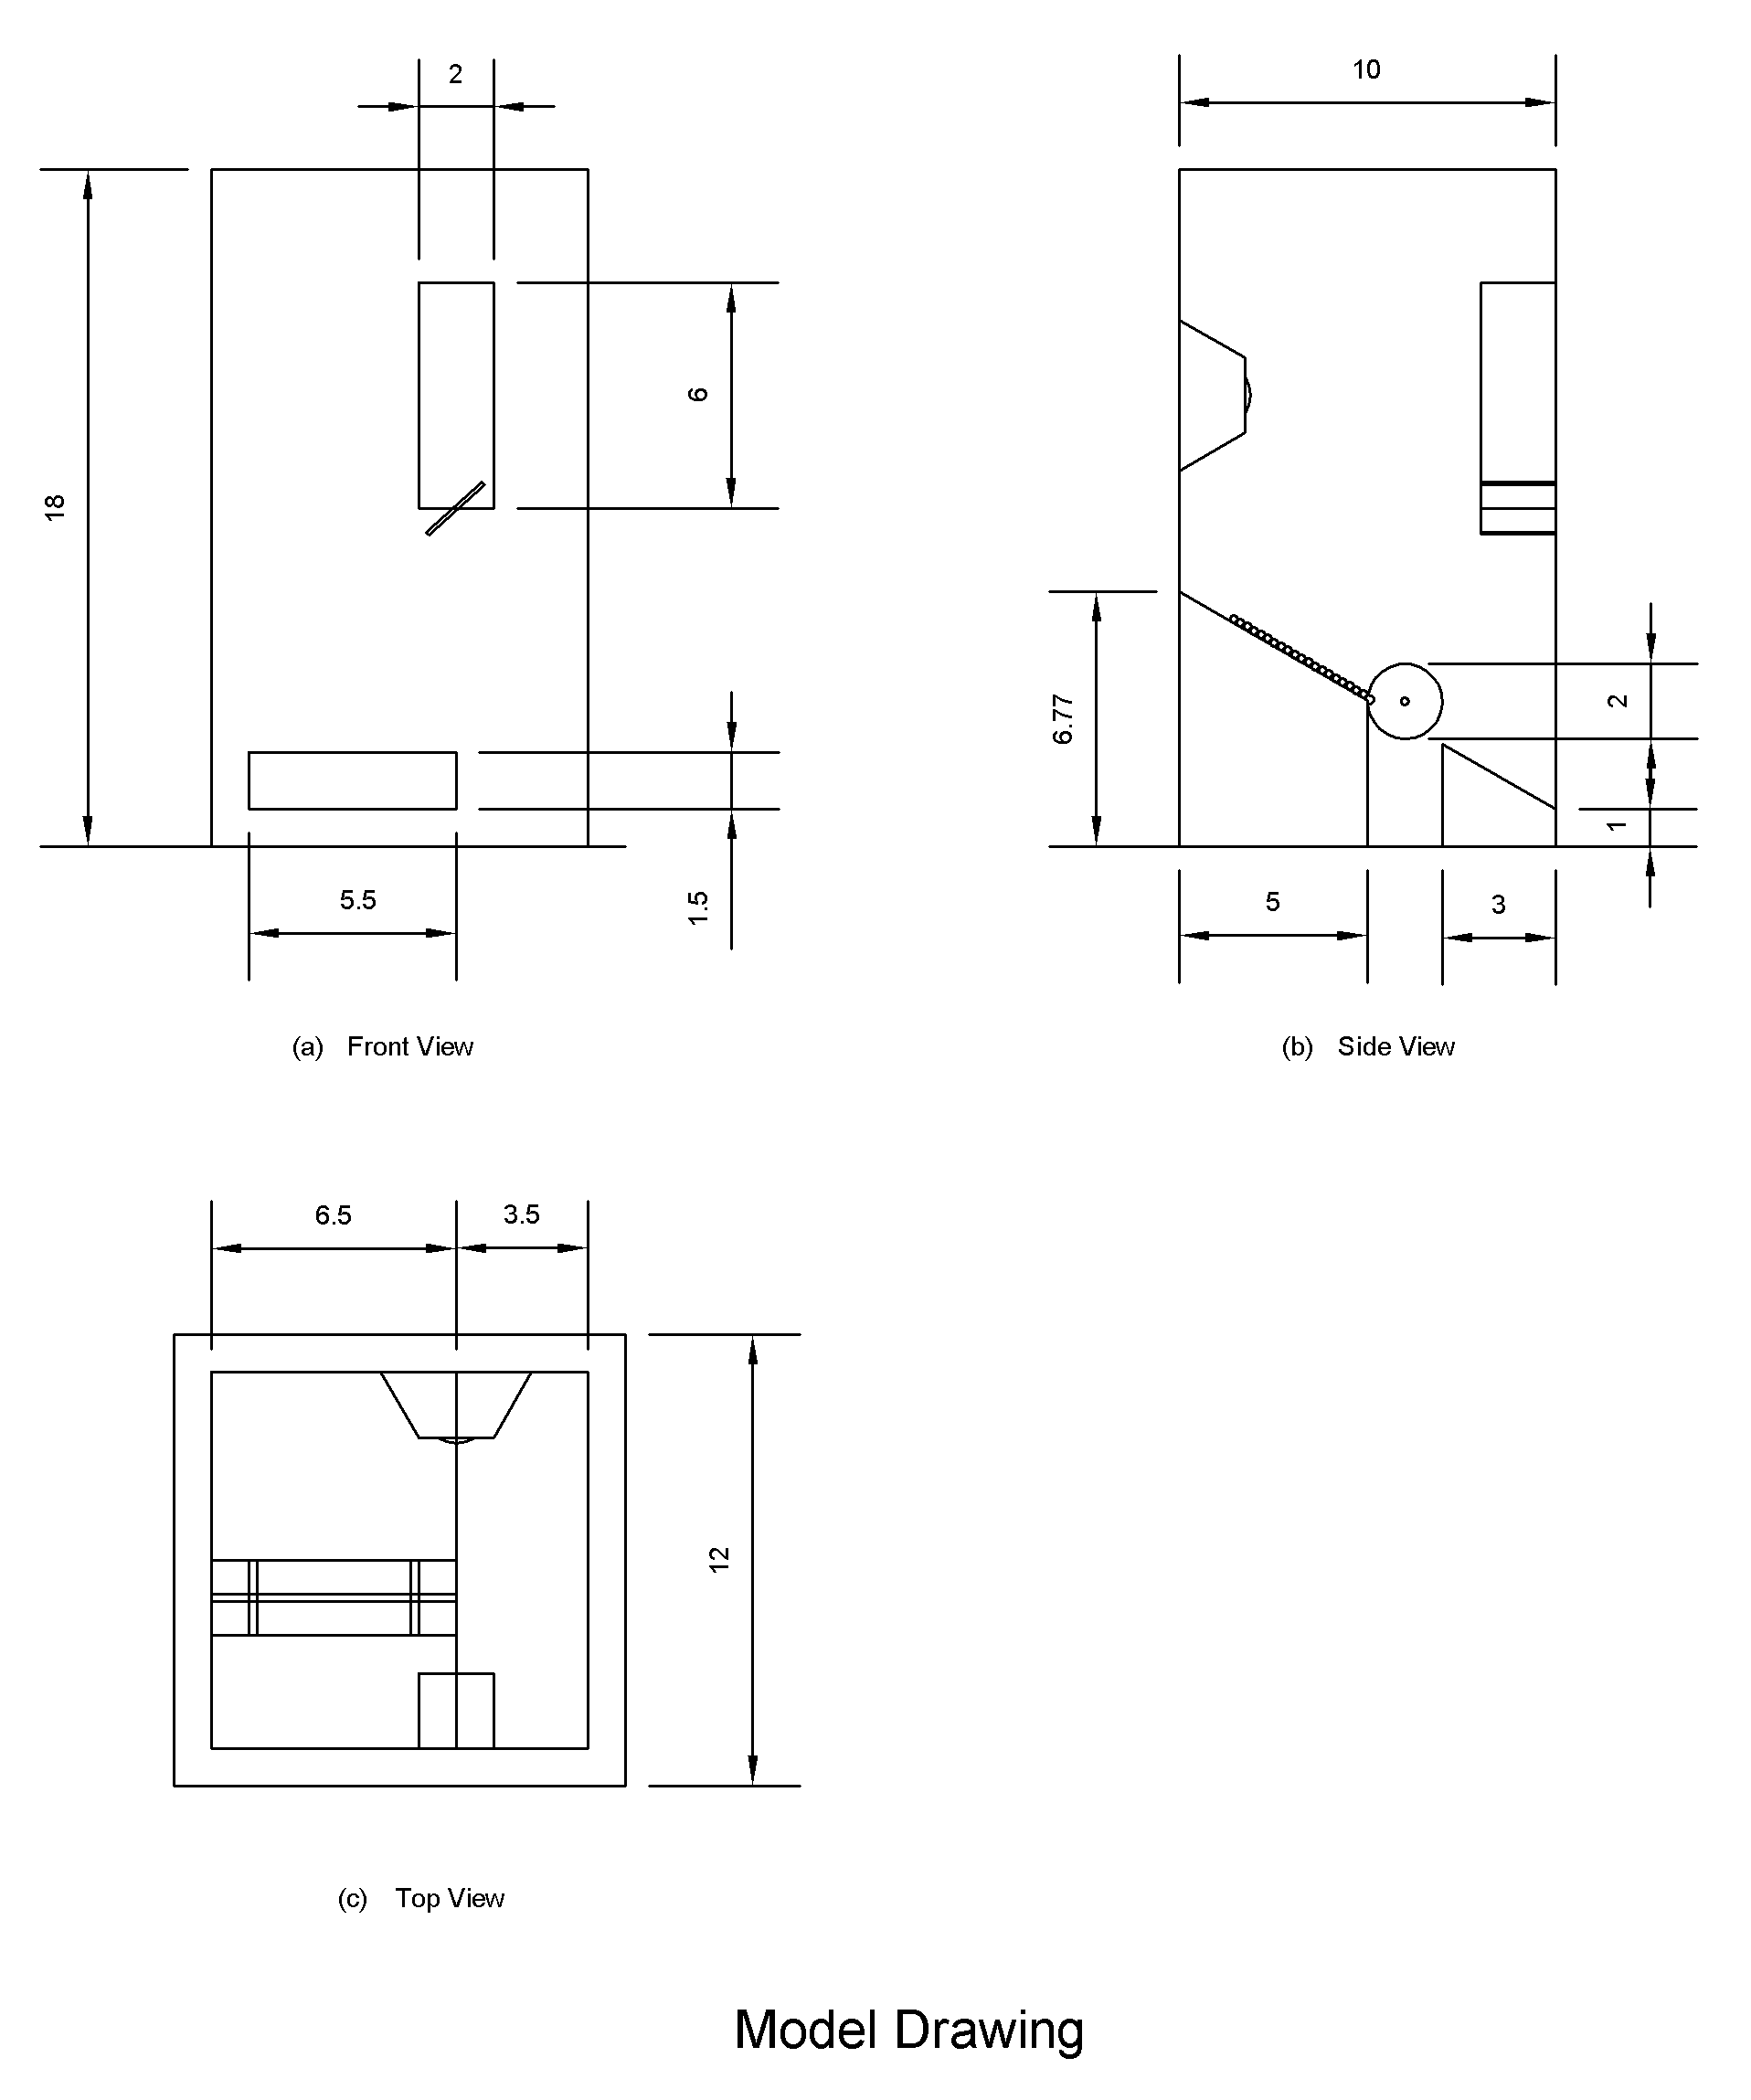
\includegraphics[width=1\linewidth]{./picture-files/model_drawing.png}
	\caption{A drawing of the proposed design (all dimensions are in inches)}
	\label{Model}
\end{figure}

\begin{figure}[H]
	\centering

	\begin{subfigure}[Isometric view] 
		{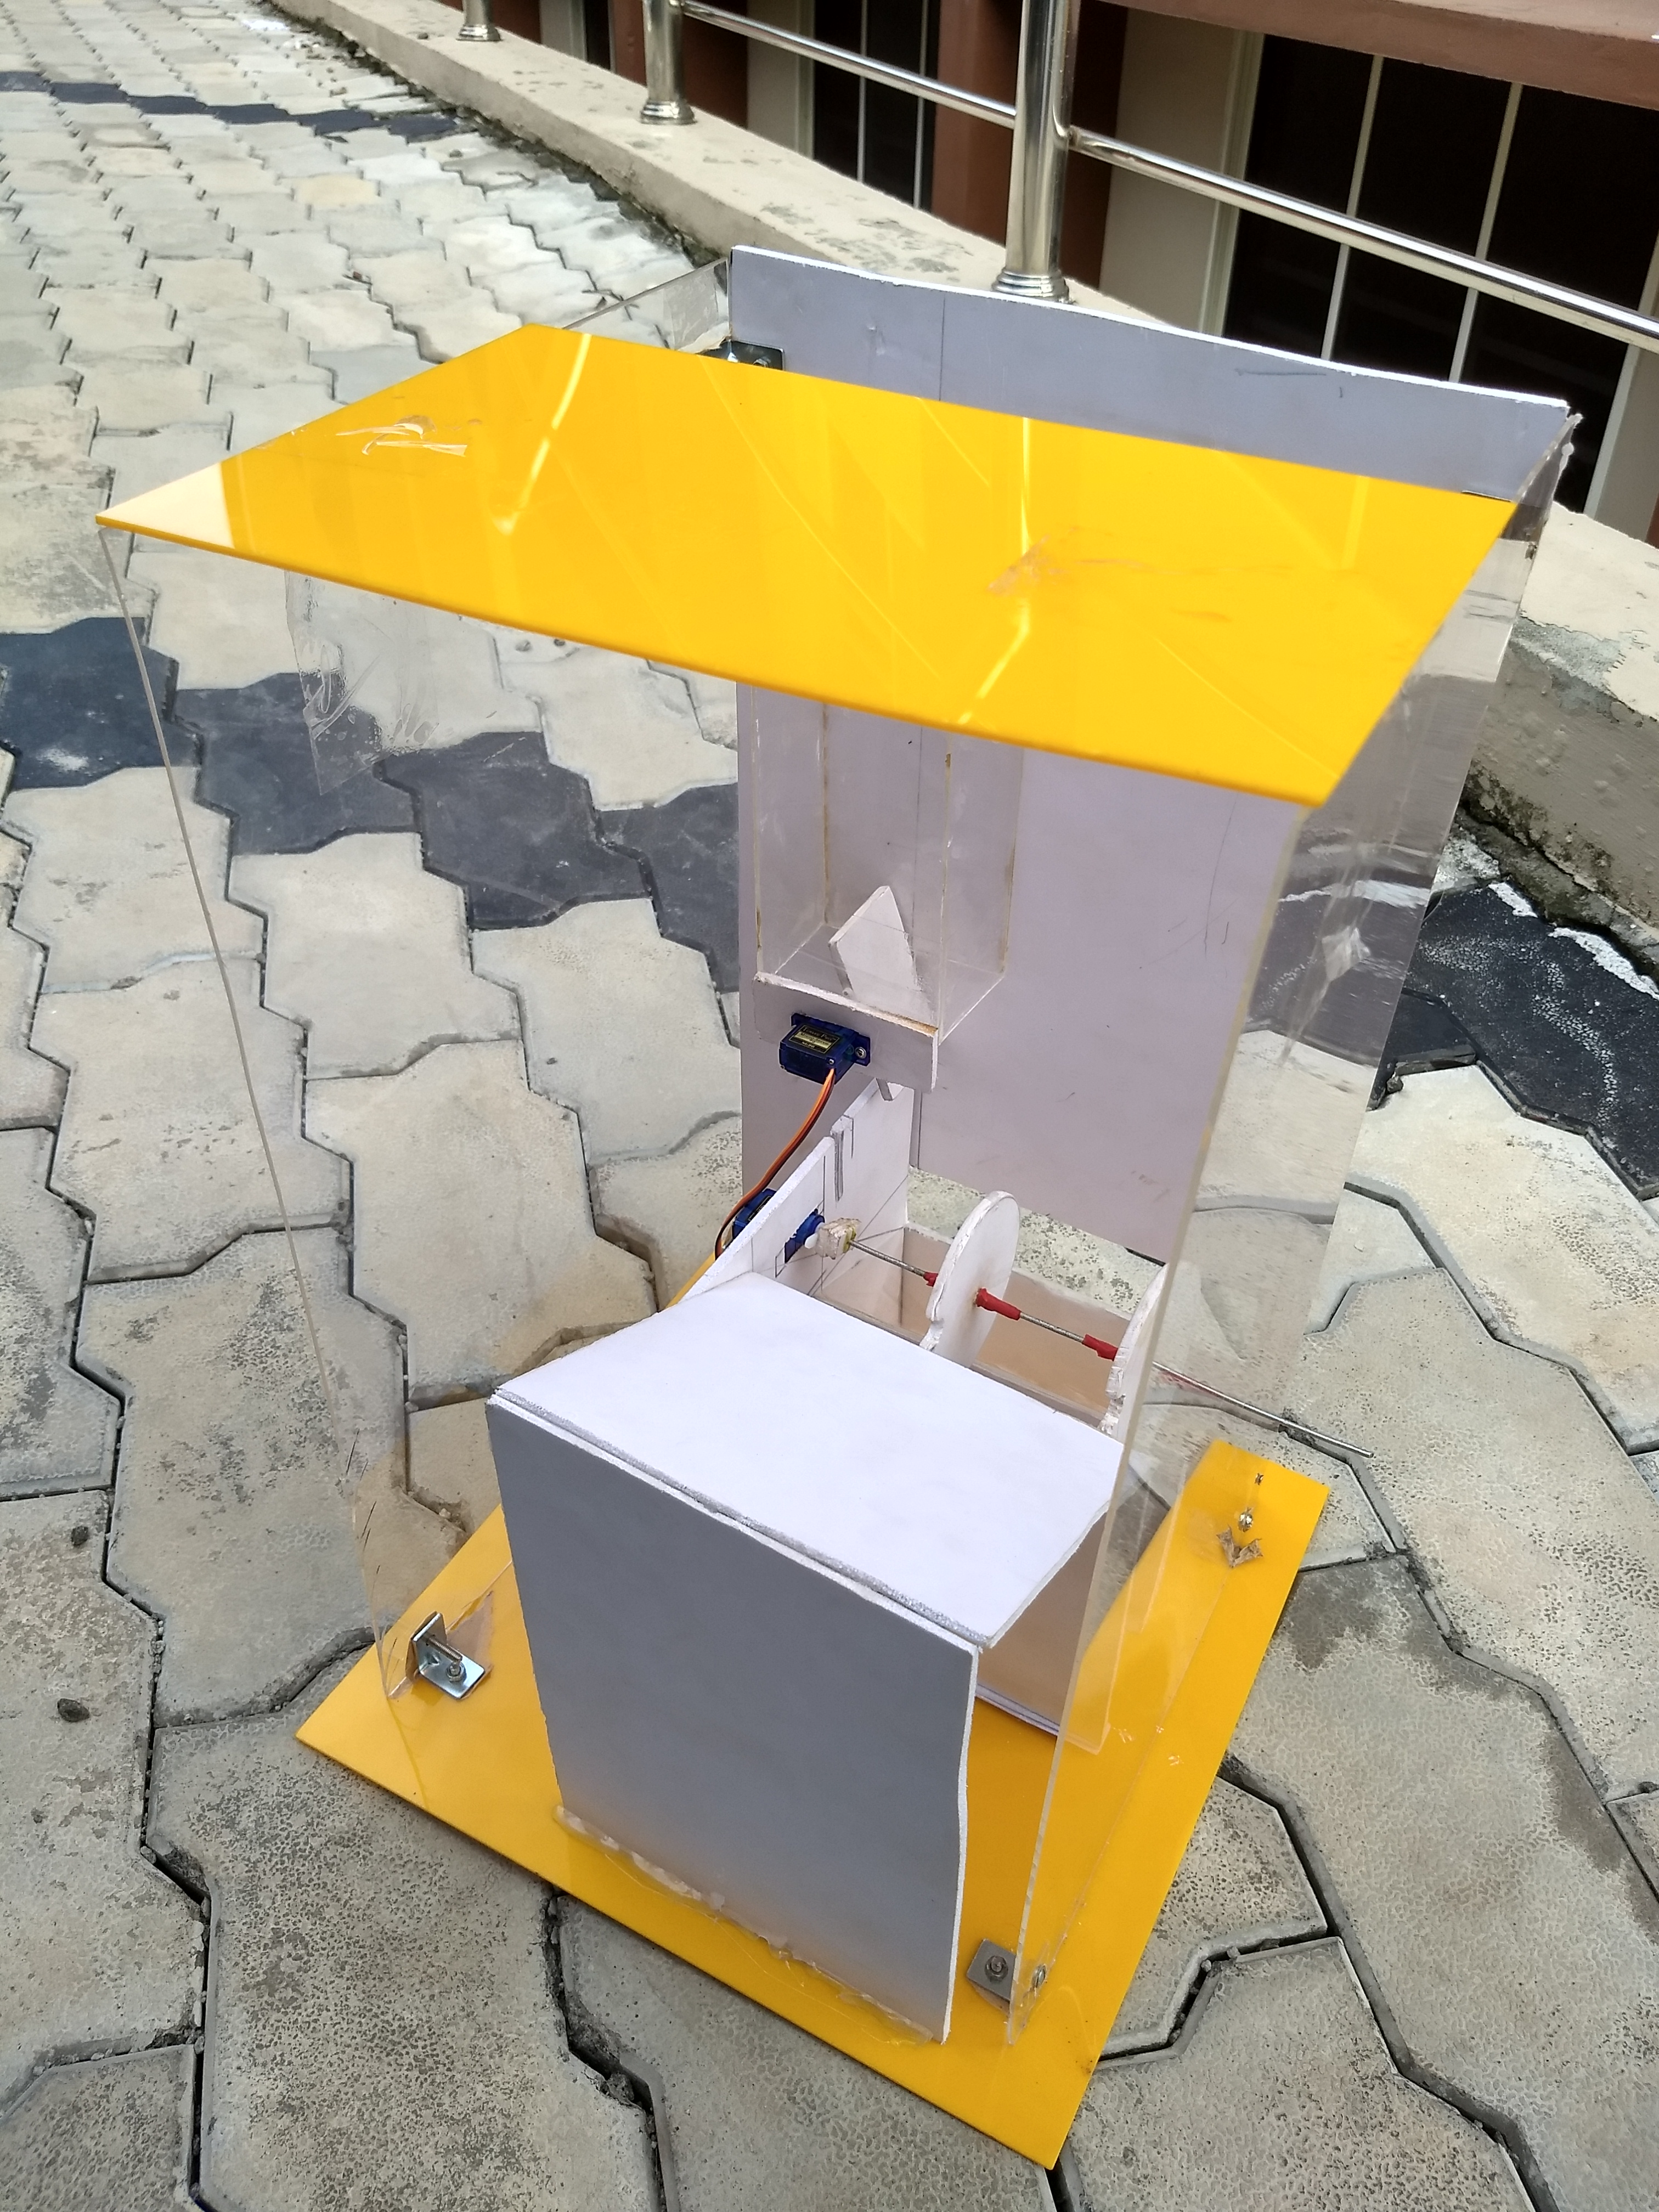
\includegraphics[width=0.45\textwidth]{./picture-files/isometric_view.jpg}}
	\end{subfigure}\hspace{1cm}
	\begin{subfigure}[Top view]
		{\includegraphics[width=0.45\textwidth]{./picture-files/top_view.jpg}}
	\end{subfigure}
	\begin{subfigure}[Side view]
	{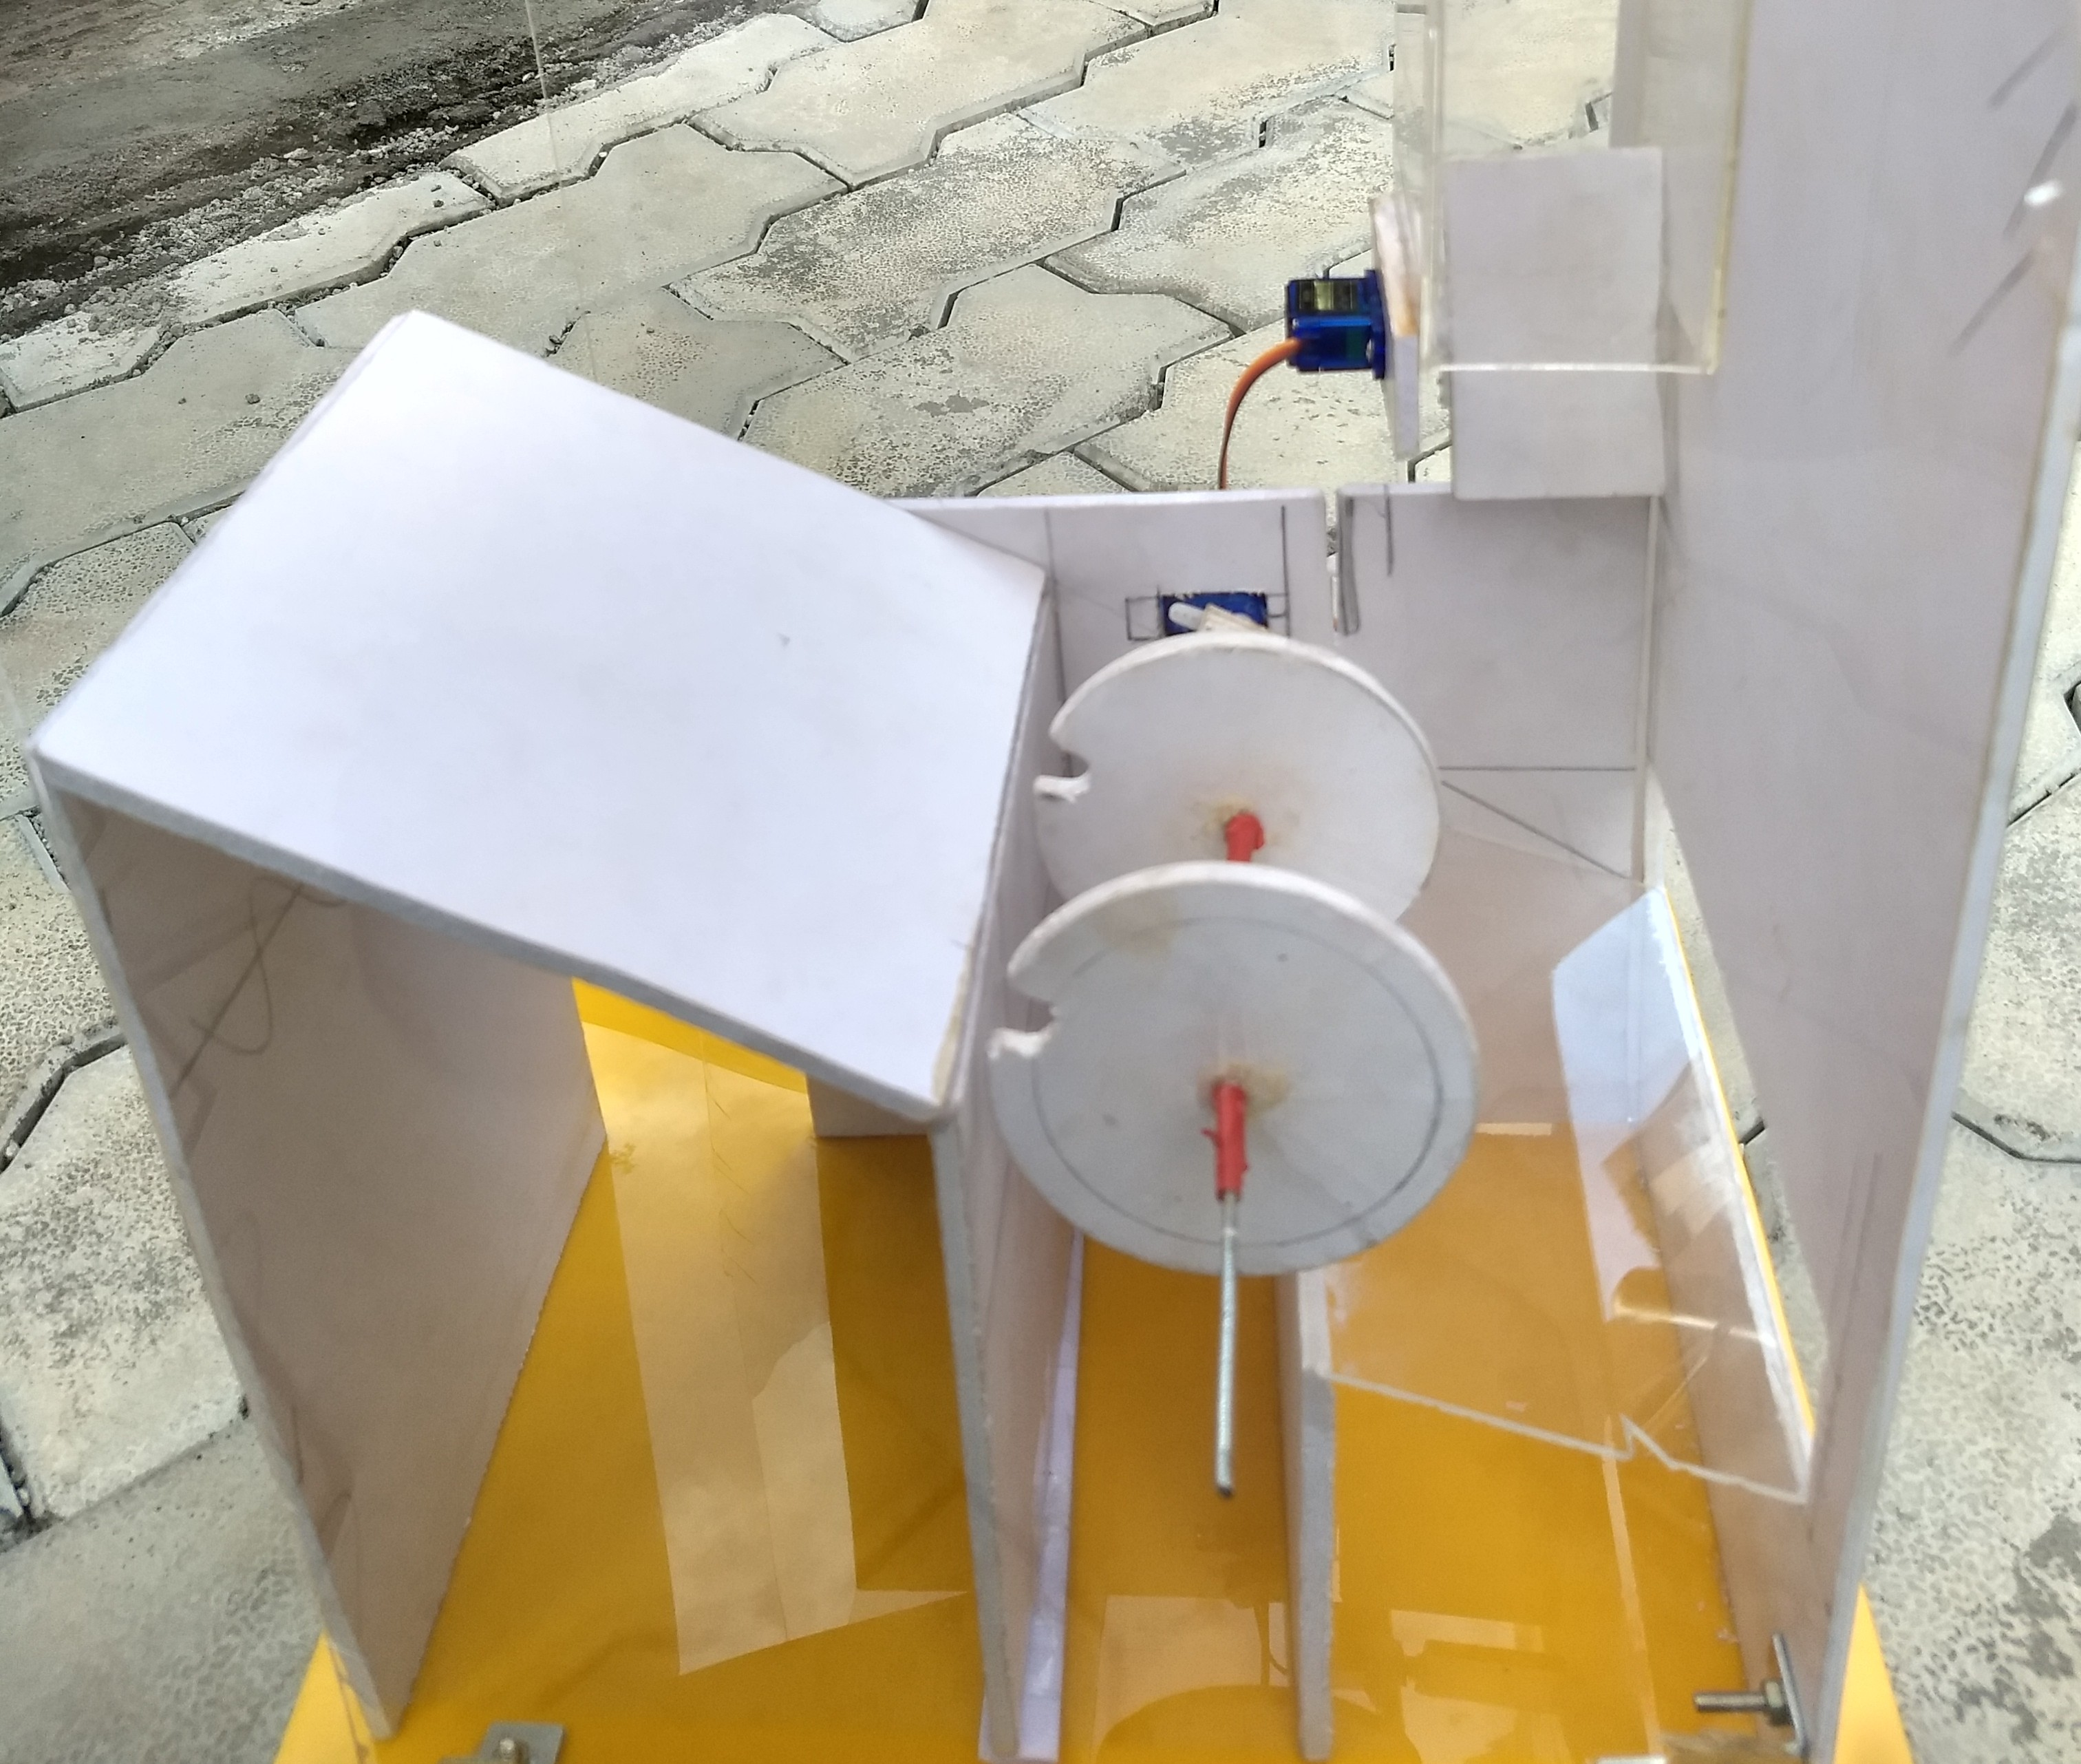
\includegraphics[width=0.7\textwidth]{./picture-files/side_view}}
	\end{subfigure}
	\caption{PPVM prototype}
	\label{proto}
\end{figure}

\section{Pen Accepting and Rejecting}
The tiltable base redirects the pen depending on whether it is a pen or not. The base is connected to a servo motor. The servo motor will turn the base left if it accepts and turns right if it rejects the deposited item. The rejected item will go out through the same ramp which is used for delivering paper pen.

\section{Rollout Mechanism}
For delivering the paper pen, a pair of circular discs are used. These discs are attached to a thin aluminum shaft which is connected to a servo motor. A small groove is cut on the outer portion of the discs, to fit just one pen. The paper pens are stacked on a ramp behind the discs. When a pen is being rolled out, the outer part of the disc prevents the stored pens from falling. The rolled-out pens fall on a ramp in front of the discs and are delivered to the user as shown in Fig \ref{rollout}

\begin{figure}[H]
	\centering
	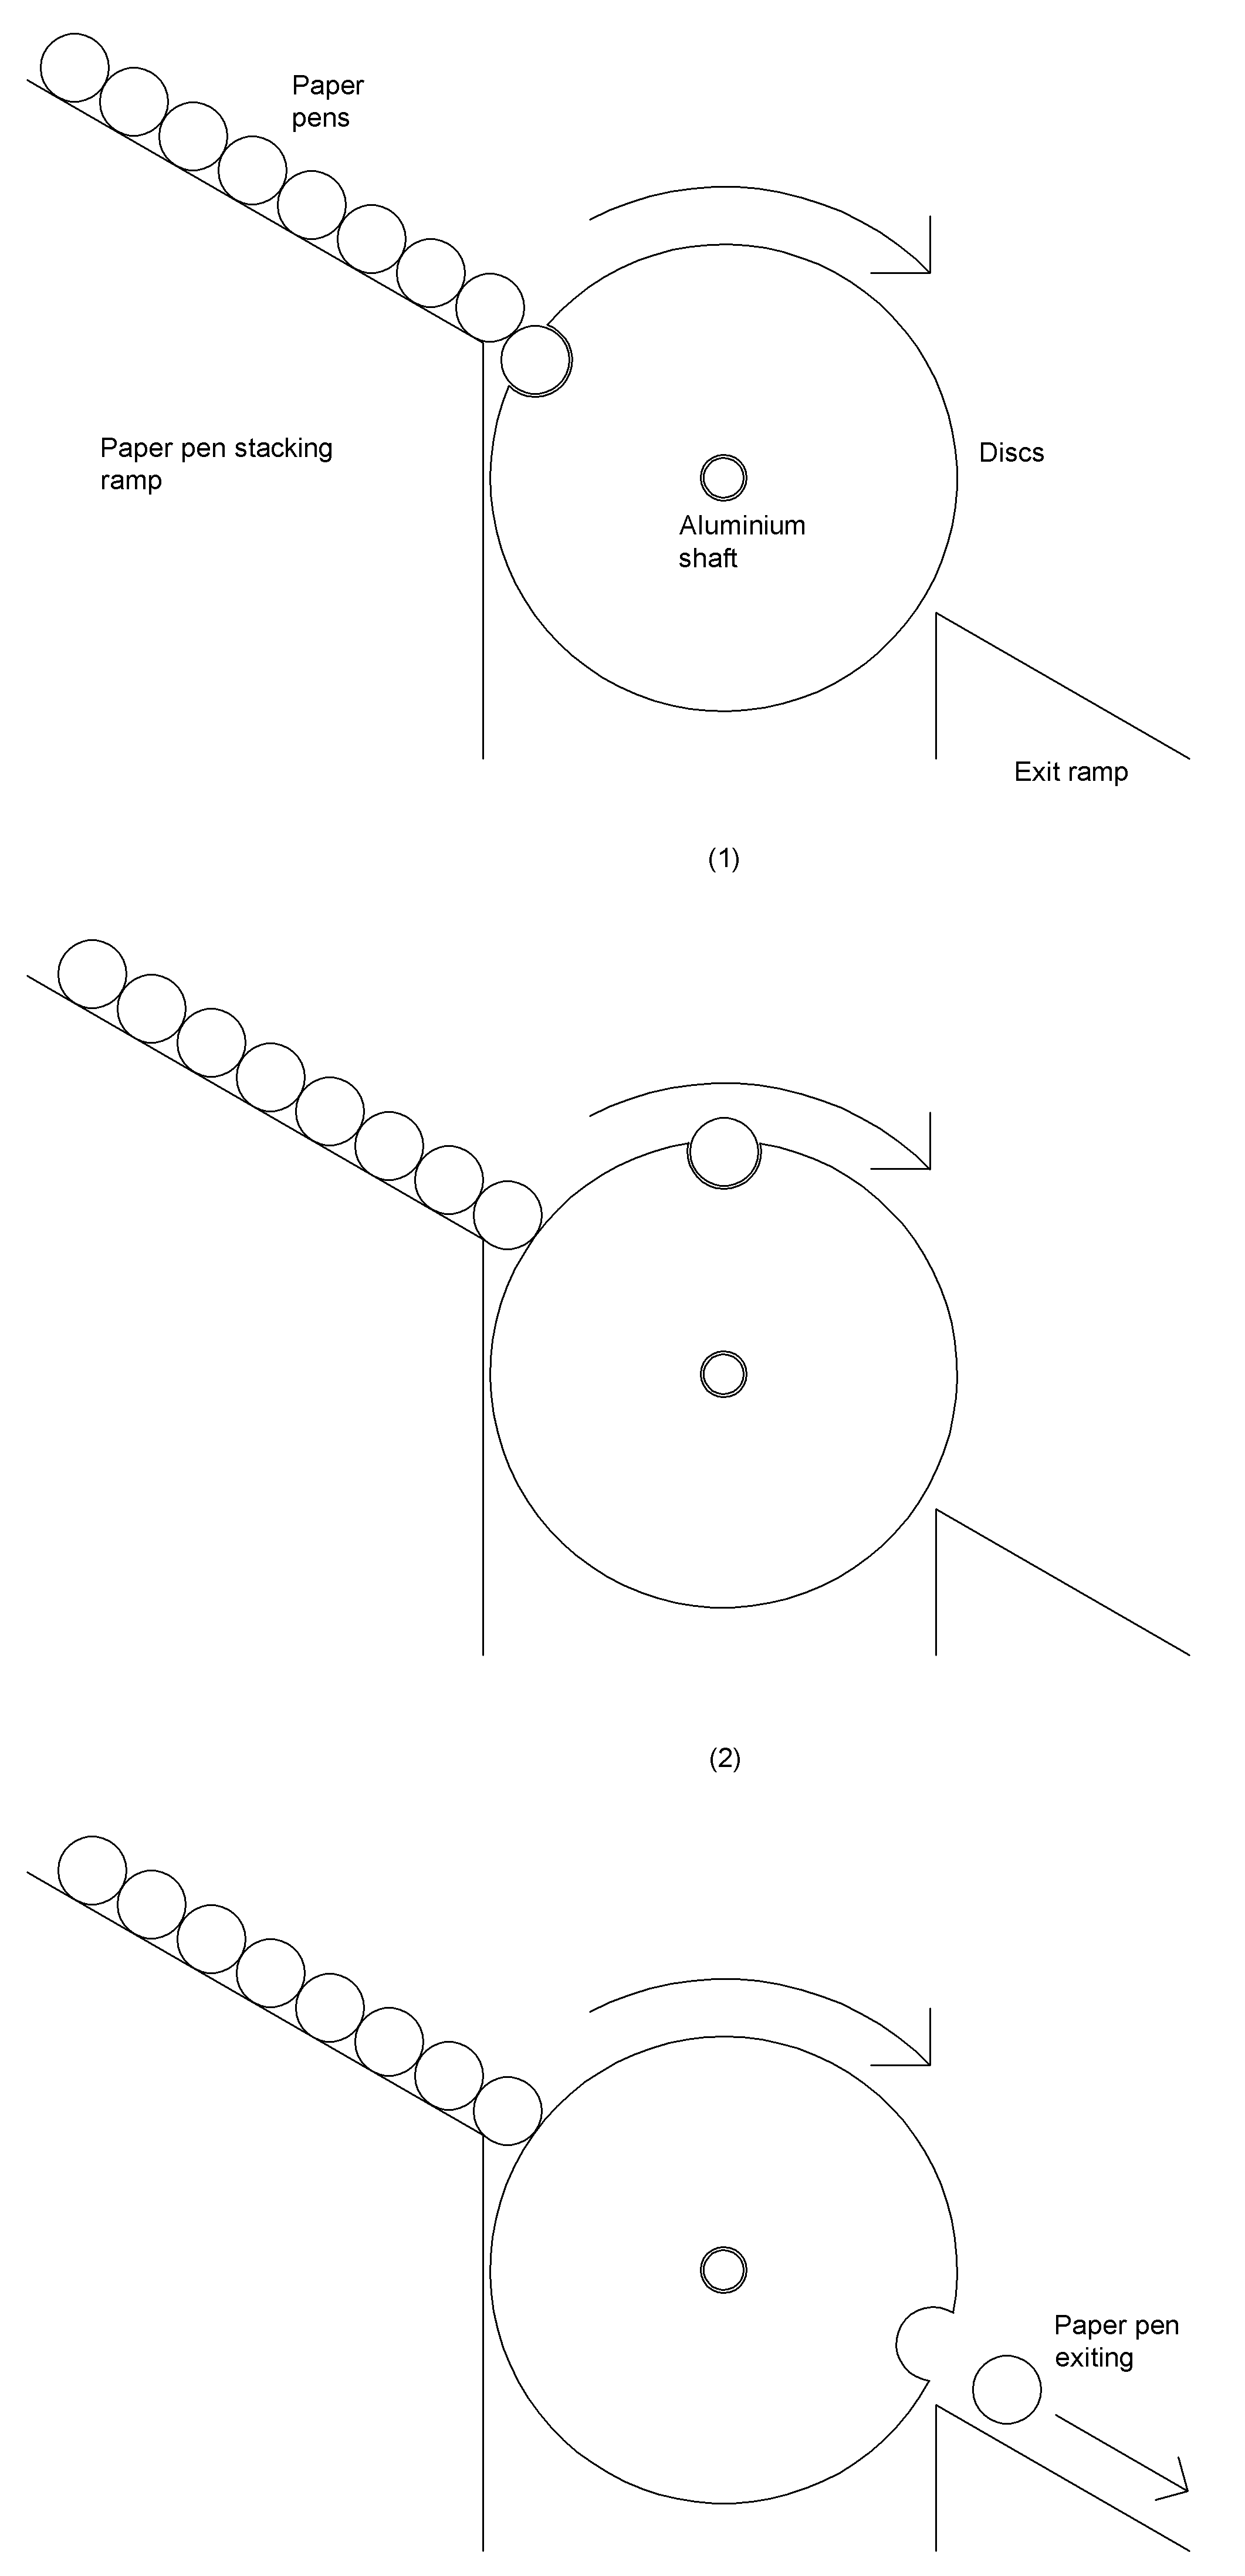
\includegraphics[width=0.6\linewidth]{./picture-files/rollout.png}
	\caption{The rollout mechanism}
	\label{rollout}
\end{figure}   

\section{Summary}

In this chapter, the main discussion was on the design of the model and its functioning. The algorithms and the procedure of operation was explained in detail. A model drawing of the prototype was also shown.